% MAIN-DOCUMENT

% Header beinhaltet Dokumentenklasse sowie includierte Packages
%KOMA-Script-Klasse: scrreprt
%deutsches Design, Schriftgröße 12, DIN A4
\documentclass[12pt,a4paper,oneside]{scrreprt}
%Seitenspiegel einstellen
\usepackage[a4paper]{geometry}
\geometry{a4paper,left=30mm,right=25mm,
bottom=20mm,top=15mm,bindingoffset=2mm,
includehead,includefoot}



%schalte Umlaute frei
\usepackage[ngerman]{babel}
%passende Codierung
\usepackage[utf8]{inputenc}
%Seitenspiegel einzustellen
\usepackage[a4paper]{geometry}
%Mathepaket
\usepackage{amsmath}
%Symbole
\usepackage{amssymb}
%griechische Symbole
\usepackage{upgreek}
%weitere Symbole
\usepackage{pxfonts}
% Phonetischen Alphabete für LaTeX
\usepackage{tipa}
%farbige Schriften
\usepackage{xcolor}
\usepackage{scrhack}
%Bilder fixieren
\usepackage{float}
%Grafiken einbinden
\usepackage{graphicx}
% Kopf- und Fußzeilen
\usepackage[automark,standardstyle,markusedcase]{scrpage2}
% deutsche Überschriften
\usepackage[ngerman]{translator}
% Kopfzeilenabstand festlegen
\setlength{\headheight}{10mm}
%Abb. statt Abbildung
\usepackage{caption3}
%klickbare Referenzen
\usepackage{hyperref}
%Quellcode Format
\usepackage{listings}
%draft Wasserzeichen
\usepackage{draftwatermark}
\SetWatermarkLightness{0.95}
\addto\captionsngerman{
\renewcommand{\figurename}{Abb.}
\renewcommand{\tablename}{Tab.}
}
%Glossar-Pakage
\usepackage[
nonumberlist, %keine Seitenzahlen anzeigen
acronym,      %ein Abkürzungsverzeichnis erstellen
toc]          %Einträge im Inhaltsverzeichnis      
{glossaries}
\usepackage{cite}
%Glossar einschalten
\makeglossaries



%Einstellungen Kopfzeile
\pagestyle{scrheadings} 
\setheadsepline{0.4pt}
\pagestyle{scrheadings}
\renewcommand*{\chapterpagestyle}{scrheadings}

%Zeilenabstand * 1.25 (default)
\renewcommand{\baselinestretch}{1.25}\normalsize


\begin{document}

% TODO: Glossar

%Titelseite

% Seitennummer aus
\thispagestyle{empty}


\begin{titlepage}

\vspace{3cm}

\begin{center}
    
\includegraphics[scale=0.8]{Titelseite/hl-logo.pdf}  
\end{center}

\vspace{2.5cm}

\begin{center}
\Large FAKULTÄT INFORMATIK
\end{center}

\vspace{1cm}
\begin{center}
    \Huge
    \textbf{Bachelorarbeit}\\
\end{center}

\vspace{1cm}

\begin{center}
    \Large
    \textsc{Programmieren in Rust und Vergleich mit C/C++}\\
\end{center}

\vspace{1.5cm}

\begin{center}
    \Large
    Thomas Keck
\end{center}

\vspace{4cm}
\begin{center}
    \large
    Betreuer: Prof. Dr. rer. nat. Dieter Nazareth
\end{center}

\end{titlepage}

\clearpage
\ifodd\count0\else
\thispagestyle{empty}
\hbox{}\newpage
\fi

%Erklärung
\thispagestyle{empty}
\vspace{15mm}
\begin{center}
\textbf{\underline{ERKLÄRUNG ZUR BACHELORARBEIT}}
\end{center}
\vspace{25mm}
\begin{center}
\large
Keck, Thomas
\end{center}
\vspace{25mm}

\begin{center}
\huge
Hochschule Landshut \\
Fakultät Informatik 
\end{center}
\vspace{10mm}

\begin{center}
\large
Hiermit erkläre ich, dass ich die Arbeit selbständig 
verfasst, noch nicht anderweitig für Prüfungszwecke 
vorgelegt, keine anderen als die angegebenen Quellen 
oder Hilfsmittel benützt, sowie wörtliche und sinngemäße 
Zitate als solche gekennzeichnet habe.  \\
\end{center}
\vspace{55mm}

\begin{center}
....................\hspace{40mm}....................................................\\

(Datum)\hspace{47mm}(Unterschrift des Studierenden)
\end{center}

\clearpage
\ifodd\count0\else
\thispagestyle{empty}
\hbox{}\newpage
\fi

% TODO: Abstract

% Liste Menüpunkte als Inhaltsverzeichnis
\tableofcontents
\setcounter{page}{1}

% Kapitel
\chapter{Einleitung}


\section{Was ist Rust?}

Rust ist eine quelloffene System-Programmiersprache, die sich auf Geschwindigkeit, Speichersicherheit und Parallelität konzentriert. Entwickler nutzen Rust für ein breites Spektrum an Anwendungsgebieten: Spiel-Engines\footnote{http://arewegameyet.com}, Betriebssysteme\footnote{z. B. Redox OS}, Dateisysteme und Browserkomponenten. \cite{Rust}

Eine aktive Gemeinschaft von Programmierern verwaltet die Codebasis und fügt fortlaufend neue Verbesserungen hinzu. Mozilla sponsert das Open-Source-Projekt.

Rust wurde von Grund auf neu aufgebaut und enthält Elemente aus bewährten und modernen Programmiersprachen. Es verbindet die ausdrucksstarke und intuitive Syntax von High-Level-Sprachen mit der Kontrolle und Leistung einer Low-Level-Sprache. Es verhindert Segmentierungsfehler und gewährleistet Threadsicherheit. Dadurch können Entwickler Code schreiben, der ehrgeizig, schnell und korrekt ist.

Rust macht die Systemprogrammierung durch die Kombination von Leistung und Ergonomie zugänglicher. Es bietet starke Features wie Zero-Cost-Abstraktionen, sichere Speicherverwaltung durch einen strengen Compiler und Typsystem sowie risikolose Nebenläufigkeit.

Große und kleine Unternehmen setzen Rust bereits ein, darunter:
\begin{itemize}
    \item Mozilla: Wichtige Komponenten von Mozilla Firefox Quantum.
    \item Dropbox: Mehrere Komponenten wurden in Rust als Teil eines größeren Projekts geschrieben, um eine höhere Effizienz des Rechenzentrums zu erreichen.
    \item Yelp: Ein Framework für Echtzeit A/B-Tests, welches auf allen Yelp-Websites und -Anwendungen verwendet wird.
\end{itemize}

\chapter{Rust toolchain}

Die Rust toolchain ist eine Sammlung von Werkzeugen, die dabei helfen, den Compiler aktuell zu halten und Projekte zu verwalten.


\section{rustup}

Das Rustup-Tool ist die empfohlene Installationsmethode für Rust. Das Tool ermöglicht zusätzlich die Verwaltung von verschiedenen Versionen, Komponenten und Plattformen. Um zwischen den Versionen stable, beta und nightly zu wechseln, kann auf der Kommandozeile eingegeben werden: \cite{RustEdition}

\begin{lstlisting}   
    rustup install beta                 # release channel
    rustup install nightly
    rustup update                       # update all channels
    rustup toolchain default nightly    # switch to 'nightly'
\end{lstlisting}

Rust unterstützt auch das Kompilieren für andere Zielsysteme, dabei kann rustup helfen. So kann man beispielsweise MUSL verwenden:

\begin{lstlisting}
    # add target
    rustup target add x86-64-unknown-linux-musl
    # build project with target
    cargo build --target=x86_64-unknown-linux-musl
\end{lstlisting}

Mit Hilfe von rustup können verschiedene Komponenten installiert werden, z.B.:

\begin{itemize}
    \item rust-docs: Lokale Kopie der Rust-Dokumentation, um sie offline lesen zu können.
    \item rust-src: Lokale Kopie des Quellcodes von Rust. Autokomplettierungs-Tools verwenden diese Information.
    \item rustfmt-preview: Zur automatischen Code-Formatierung.
\end{itemize}

\begin{lstlisting}
    rustup component add rustfmt-preview
\end{lstlisting}


\section{rustc}

Der Compiler von Rust, er übersetzt den Quellcode in einen binären code, entweder als Bibliothek oder als ausführbare Datei. Die meisten Rust-Programmierer rufen rustc nicht direkt auf, sondern indirekt über Cargo. \cite{RustcBook}

\subsection{Grundlegende Verwendung}

Der Kommandozeilenbefehl für das Kompilieren mit rustc ähnelt dem eines C-Programms:

\begin{lstlisting}
    gcc   hello.c  -o helloC            # C program
    rustc hello.rs -o helloRust         # Rust program
\end{lstlisting}

Anders als in C muss nur der crate root\footnote{Quellcode-Datei mit der main() Methode} angegeben werden. Der Compiler kann mithilfe des Codes selbständig festellen, welche Dateien er übersetzen und linken muss. Es müssen somit keine Objektdateien erstellt werden.

\subsection{Lints}

Ein Lint ist ein Werkzeug, das zur Verbesserung des Quellcodes verwendet wird. Der Rust-Compiler enthält eine Reihe von Lints. Beim Kompilieren werden dadurch Warnungen oder Fehlermeldungen ausgeben. Beispiel:

\begin{lstlisting}
    $ cat main.rs
    fn main() {
        let x = 5;
    }

    $ rustc main.rs
    warning: unused variable: `x`
     --> main.rs:2:9
      |
    2 |     let x = 5;
      |         ^ help: consider using `_x` instead
      |
      = note: #[warn(unused_variables)] on by default
\end{lstlisting}

Das ist das \glqq unused\_variables\grqq{} Lint. Es besagt, dass eine Variable eingeführt wurde, die nicht im Code verwendet wurde. Dies ist nicht falsch, es könnte jedoch ein Bug sein.


\section{Cargo}

Cargo ein Projektmanager für Rust. Damit können Abhängigkeiten heruntergeladen und verteilbare Pakete erstellt werden, welche auf crates.io\footnote{Paketeregister der Rust-Community} hochgeladen werden können. \cite{CargoBook}

\subsection{Projektverwaltung}

Projekte können mit Hilfe von Cargo erstellt werden, dabei entsteht eine bestimmte Ordnerstruktur mit einer Cargo.toml Datei sowie dem crate root im src-Ordner. Ein Projekt kann eine Applikation (binary) oder eine Bibliothek (library) sein. Der crate root ist bei einer Applikation immer \glqq main.rs\grqq{} und bei einer Bibliothek \glqq lib.rs\grqq{}.

\begin{lstlisting}[style=tree]
    $ cargo new hello_world --bin       # --lib for library
         Created binary (application) `hello_world` package

    $ cd hello_world
    $ tree .
    .
    ├── Cargo.toml
    └── src
        └── main.rs
    
    1 directory, 2 files
\end{lstlisting}

Die Cargo.toml enthält alle wichtigen Metainformationen, die Cargo zum Kompilieren benötigt. 

\begin{lstlisting}
    [package]
    name = "hello_world"
    version = "0.1.0"
    authors = ["Thomas Keck <s-tkeckk@haw-landshut.de>"]
    edition = "2018"
    
    [dependencies]    
\end{lstlisting}

Die Informationen über den Author enthält Cargo von den Umgebungsvariablen CARGO\_NAME und CARGO\_EMAIL. In Rust gibt es sogenannte editions, welche in der Regel in einem zeitlichen Abstand von zwei oder drei Jahren veröffentlicht werden und, ähnlich wie in C, einen Standard festlegen. Zum Zeitpunkt der Erstellung dieser Arbeit gibt es zwei Editionen: 2015 und 2018. Das Pendant in C wären die C-Standards wie z.B. C90, C99 oder C11.

Zudem können hier zusätzliche Bibliotheken angegeben werden, die Cargo automatisch von crates.io herunterlädt in in das Projekt einbindet. Cargo erstellt für genauere Informationen der Abhängigkeiten eine Datei Cargo.lock, diese sollte nicht manuell verändert werden, da sie von Cargo gepflegt wird. Mithilfe von Cargo können Tests gestartet werden, genauere Information dazu sind aus Kapitel 3.6 zu entnehmen.

\subsubsection{Projekt-Layout}

\begin{figure}[htbp]
    \centering
    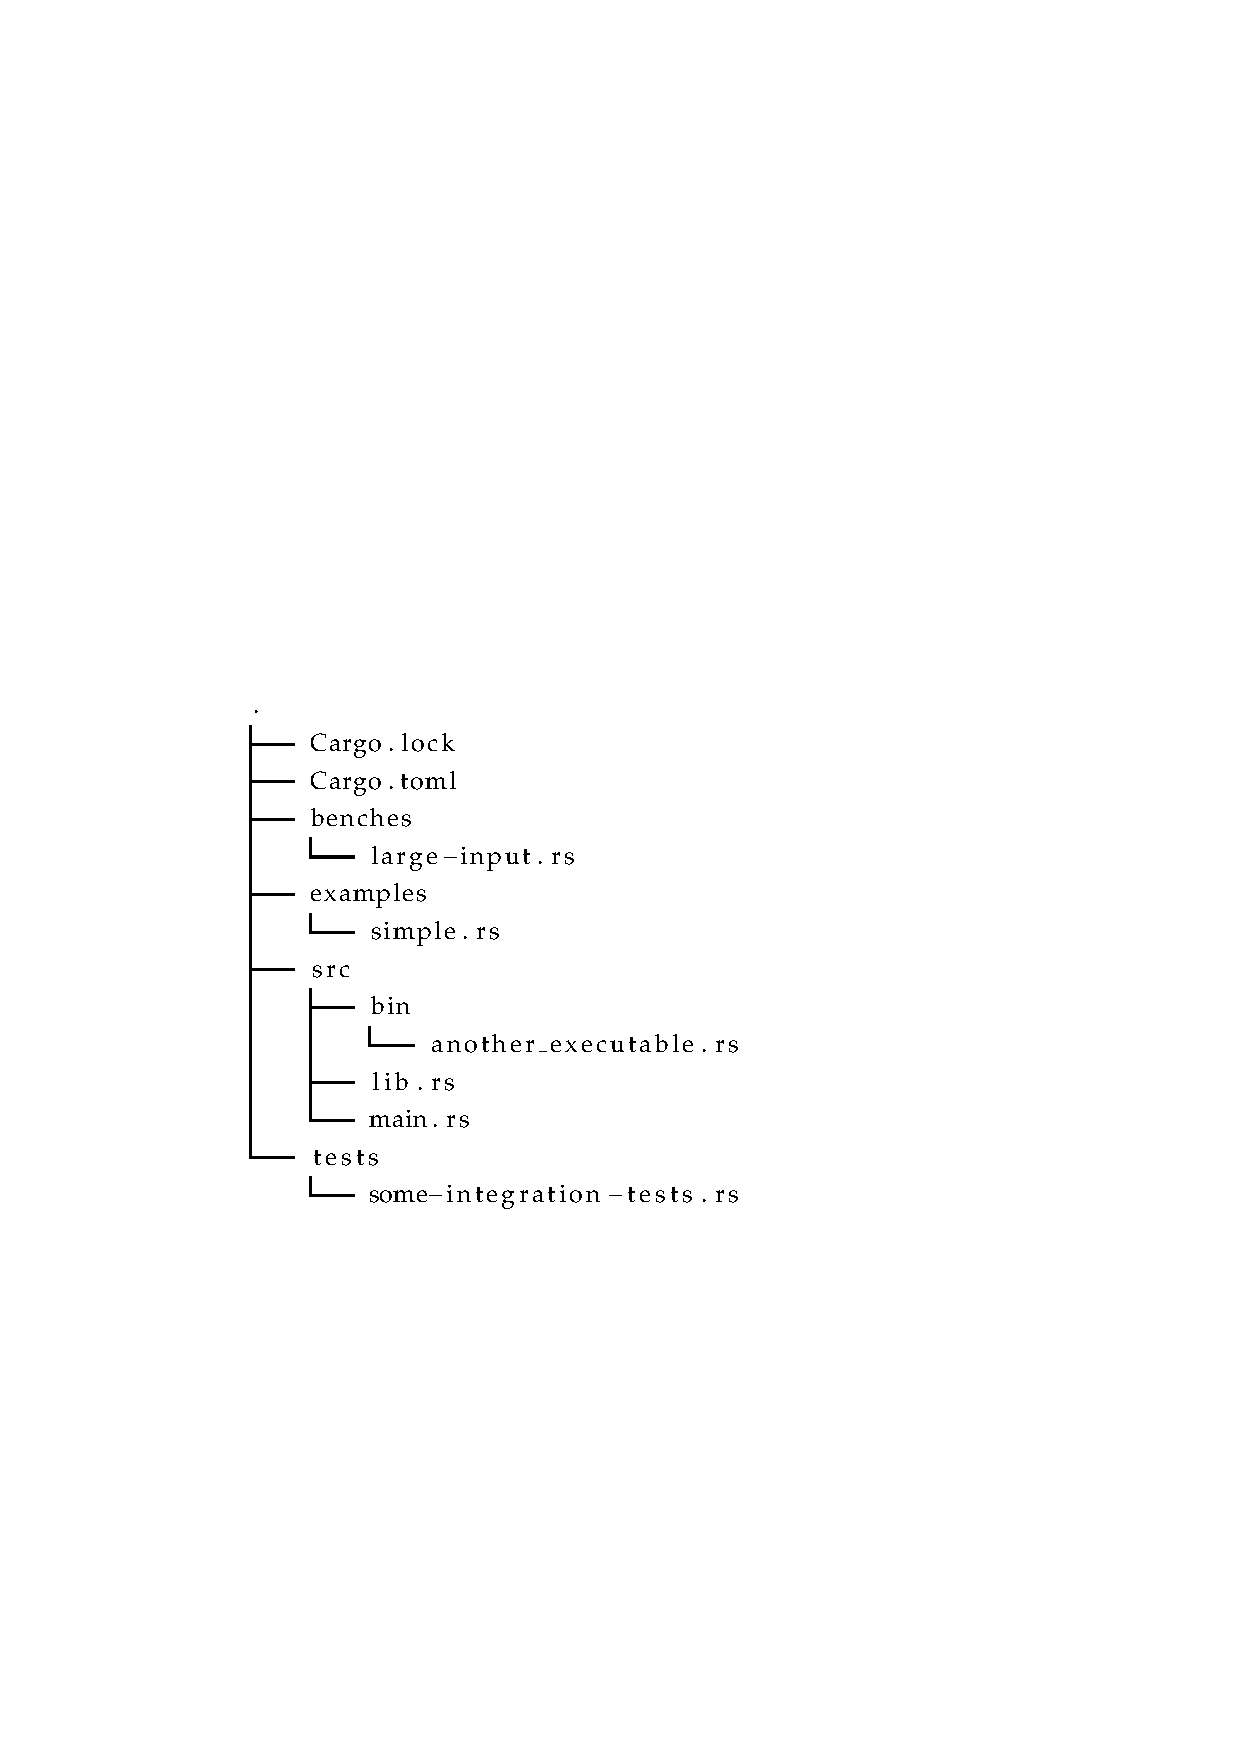
\includegraphics{Toolchain/dateibaum.pdf}
    \caption{Dateibaum eines Rust Projekts}
\end{figure}

\begin{itemize}
    \item Cargo.toml und Cargo.lock werden im Wurzelverzeichnis des Projekts gespeichert
    \item Quellcode-Dateien sind im src-Ordner vorgesehen
    \item Die Standarddatei für Bibliotheken ist src/lib.rs
    \item Die Standarddatei für ausführbare Programme ist src/main.rs
    \item Quellcode für sekundäre ausführbare Programme src/bin/*.rs
    \item Integrationstests im Ordner tests, Unit-Tests werden in die jeweilige Programmdatei geschrieben
    \item Beispiele im examples Ordner
    \item Benchmarks im benches Ordner
\end{itemize}

\subsubsection{Wichtige Kommandozeilenbefehle für Cargo}

Zum Kompilieren uns Ausführen:

\begin{lstlisting}
    $ cargo build
    $ ./target/debug/hello_world

    $ cargo build --release             # optimized performance
    $ ./target/release/hello_world

    # alternative as one command
    $ cargo run
\end{lstlisting}

Zum Testen:

\begin{lstlisting}
    # run all standard tests
    $ cargo test

    # run all tests marked as ignored
    $ cargo test -- --ignored
\end{lstlisting}

\subsection{Veröffentlichung bei crates.io}

Das Paketeregister der Rust-Community, genannt crates.io, ist ein Ort für Bibliotheken, die von verschiedenen Programmierern aus der Community verwaltet werden. Eine Veröffentlichung ist permanent. Das heißt, dass keine Versionsnummern überschrieben werden können und somit der Code nicht gelöscht werden kann. Jedoch gibt es keine Begrenzung für die Anzahl der Versionen, die veröffentlicht werden können.

Vor der Veröffentlichung wird ein Account benötigt. Dazu muss mit einem Github-Account auf crates.io ein API-Token generiert werden. Danach kann man sich über einen Befehl auf der Kommandozeile anmelden:

\begin{lstlisting}
    $ cargo login abcdefghijklmnopqrstuvwxyz012345
\end{lstlisting}

Dieser Token wird anschließend in einem lokalen Verzeichnis gespeichert und sollte nicht mit anderen geteilt werden. Erneute Generierung eines Tokens ist möglich.

Mithilfe von Cargo werden eigene Bibliotheken paketiert, dabei entsteht eine *.crate-Datei im Unterverzeichnis target/package.

\begin{lstlisting}
    $ cargo package
\end{lstlisting}

Dabei ist zu beachten, dass es eine Beschränkung der Uploadgröße von 10 MB für *.crate-Dateien gibt. Um die Dateigröße einzuschränken, können Dateien exkludiert bzw. inkludiert werden, dazu stehen die Schlüsselwörter \glqq exclude\grqq{} (blacklisting) und \glqq include\grqq{} (whitelisting) in der Cargo.toml-Datei zur Verfügung:

\begin{lstlisting}
    [package]
    # ...
    exclude = [
        "public/assets/*",
        "videos/*",
    ]
\end{lstlisting}

bzw.

\begin{lstlisting}
    [package]
    # ...
    include = [
        "**/*.rs",
        "Cargo.toml",
    ]
\end{lstlisting}

Zu beachten ist, dass das Schlüsselwort \glqq include\grqq{}, wenn gesetzt, \glqq exclude\grqq{} überschreibt.

Zum Hochladen muss nur noch folgender Befehl ausgeführt werden:

\begin{lstlisting}
    $ cargo publish
\end{lstlisting}

Dieser Befehl paketiert die Bibliothek automatisch, falls keine lokale crate-Datei gefunden wurde.

Zum Veröffentlichen einer neuen Version muss lediglich die Versionsnummer in der Cargo.toml verändert werden.

\subsubsection{Verwalten eines crate.io basierten Pakets}

Die Verwaltung eines Pakets geschieht in Rust primär auf der Kommandozeilenebene mit Cargo.

Wenn ein schwerwiegender Bug in einem bereits hochgeladenen Paket gefunden wurde, kann diese Version aus dem Index von crates.io entfernt, jedoch nicht gelöscht werden.

\begin{lstlisting}
    $ cargo yank --vers 1.0.1
    $ cargo yank --vers 1.0.1 --undo    # undo the yank
\end{lstlisting}

Diese Pakete können immer noch heruntergeladen und in andere Projekte eingebunden werden, die bereits an \glqq yanked\grqq{} Pakete gebunden waren. Cargo lässt dies dies nicht bei neu erstellten Crates\footnote{Bibliothek oder Paket in Rust} zu.

Ein Projekt wird meist von mehreren Entwicklern programmiert oder Besitzer des Projekts ändert sich im Laufe der Zeit. Folgende Befehle fügen neue Entwickler zu einem Projekt hinzu, welche dann in der Lage sind, auf crates.io zu veröffentlichen bzw. entfernen sie aus dem Projekt:

\begin{lstlisting}
    # "named" owner:
    $ cargo owner --add my-buddy
    $ cargo owner --remove my-buddy

    # "team" owner:
    # syntax: github:org:team
    $ cargo owner --add github:rust-lang:owners
    $ cargo owner --remove github:rust-lang:owners
\end{lstlisting}

Wenn ein Teamname angegeben wird, sind diese nicht befugt, neue \glqq owner\grqq{} hinzuzufügen. Die Befehle yank und publish sind Teams jedoch erlaubt. Ist ein \glqq named owner\grqq{} in einem Team, so sind alle Entwickler eines Teams als \glqq named owner\grqq{} eingestuft.

\subsection{Externe Tools}

Cargo versucht, die Integration von Tools von Drittanbietern zu vereinfachen, z.B. für IDEs oder anderen Build-Systemen. Dazu verfügt Cargo über mehrere Möglichkeiten:

\begin{itemize}
    \item cargo metadata-Befehl
    \item message-format Argument
    \item benutzerdefinierte Befehle
\end{itemize}

\subsubsection{Information über die Paketstruktur mit cargo metadata}

\begin{lstlisting}
    $ cargo metadata
\end{lstlisting}

Dieser Befehl gibt im JSON-Format alle Metadaten über ein Projekt aus. Darunter Befinden sich die Version des aktuellen Projekts sowie eine Liste der Pakete und Abhängigkeiten. Grobe Struktur:

\begin{lstlisting}
    {
        "version": integer,
        "packages": [ {
            "id": PackageId,
            "name": string,
            "version": string,
            "source": SourceId,
            "dependencies": [ Dependency ],
            "targets": [ Target ],
            "manifest_path": string,
        } ],
        "workspace_members": [ PackageId ],
        "resolve": {
            "nodes": [ {
                "id": PackageId,
                "dependencies": [ PackageId ]
            } ]
        }
    }
\end{lstlisting}

\subsubsection{Informationen beim Kompilieren}

Mit dem Argument \glqq message-format\grqq{} können genauere Informationen beim Kompilieren herausgefiltert werden:

\begin{lstlisting}
    $ cargo build --message-format=json
\end{lstlisting}

Dadurch entsteht ein Output im JSON-Format mit Informationen über Compiler-Fehlermeldungen und -Warnungen, erzeugte Artefakte und das Ergebnis.

\subsubsection{Benutzerdefinierte Befehle}

Cargo ist so ausgelegt, dass es erweitert werden kann, ohne dass Cargo selbst modifiziert werden muss. Dazu muss ein Programm in der Form cargo-\textit{command} in einem der \$PATH-Verzeichnisse des Benutzers liegen. Anschließend kann es von Cargo aufgerufen werden mit \glqq cargo \textit{command}\grqq{}.Wenn ein solches Programm von Cargo aufgerufen wird, übergibt es, wie es üblich ist, als ersten Parameter den Programmnamen. Als zweites die Bezeichnung des Programms (\textit{command}). Alle weiteren Parameter in der Befehlszeile werden unverändert weitergeleitet.

Beispiel:

\begin{lstlisting}
    // cargo-listargs
    use std::env;

    fn main() {
        let args: Vec<_> = env::args().collect();
        println!("{:?}", args);
    }
\end{lstlisting}

Obiges Programm gibt eine Liste der Parameter aus, die übergeben wurden. Es könnte auch in C programmiert sein, entscheidend ist, dass der Programmname in der richtigen Form ist.

\begin{lstlisting}
    $ ./cargo-listargs arg1 arg2
    # ["./cargo-listargs", "arg1", "arg2"]

    $ cargo listargs arg1 arg2
    # ["path/to/cargo-listargs", "listargs", "arg1", "arg2"]
\end{lstlisting}

Im Internet gibt es zum Zeitpunkt der Erstellung dieses Dokuments bereits über 40 benutzerdefinierte Befehle, die von der Rust-Community erstellt wurden. \cite{CargoSubcommands}


% BibTex mit Stil alpha
\nocite{*}
\bibliography{Bibliothek}{}
\bibliographystyle{alpha}

% Abbildungsverzeichnis, Tabellenverzeichnis und Glossar ausgeben
\listoffigures
\listoftables
\printglossaries 

\end{document}
